\documentclass[oneside, titlepage, 12pt, a4paper]{report}

\usepackage{amsmath}	% align
\usepackage{amsfonts}	% \mathbb
\usepackage{amssymb}	% \mathcal
\usepackage{mathtools}	% \norm definiálás
\usepackage[magyar]{babel}	% tartalomjegyzék felirat
\usepackage[utf8]{inputenc}	% magyar karakterek
\usepackage[T1]{fontenc}
\usepackage{graphicx}	% ábrák
\usepackage{setspace}	% sorköz \onehalfspacing

\newtheorem{theorem}{Tétel}[section]
\newtheorem{lemma}{Lemma}[section]
\newtheorem{definition}{Definíció}[section]
\newtheorem{statement}{Állítás}[section]

\DeclareMathOperator{\Ima}{Im}	% képtér operátor
\DeclareMathOperator{\Ker}{Ker}	% magtér operátor
\DeclareMathOperator{\Dom}{Dom}	% értelmezési tartomány operátor
\DeclareMathOperator{\coker}{coker}	% magtér operátor
\DeclareMathOperator{\codim}{codim}	% kodimenzió operátor
\DeclareMathOperator{\ind}{ind}	% index operátor
\DeclareMathOperator{\Span}{span}	% kifeszített tér

\DeclarePairedDelimiter\norm{\lVert}{\rVert}	% norma
\DeclarePairedDelimiter\abs{\lvert}{\rvert}	% abszolút érték - abs* kell megfelelő mérethez


\textwidth=6.truein \textheight=9.truein
\hoffset=-.5truein
\voffset=-.8truein

\begin{document}
\begin{titlepage}
% belső fedőlap

% minta forrása: https://github.com/shdnx/ELTE-LaTeX-Thesis-Base
\begin{minipage}{0.40\linewidth}

\includegraphics[scale=0.8]{./abrak/elte_logo_szines.jpg}
\end{minipage}
\begin{minipage}{0.50\linewidth}
\begin{center}
Eötvös Loránd Tudományegyetem \\
Informatikai Kar \\
Numerikus Analízis Tanszék
\end{center}
\end{minipage}

\hrule
\vfill

\begin{center}
\Huge
\textbf{A Ljapunov-Schmidt-módszer}
\normalsize
\end{center}

\vfill

\begin{minipage}[t]{0.5\linewidth}
\begin{flushleft}
\textbf{Dr. Kovács Sándor} \\
Adjunktus
\end{flushleft}
\end{minipage}
\begin{minipage}[t]{0.5\linewidth}
\begin{flushright}
\textbf{Lipták Bence Gábor} \\
Programtervező Informatikus MSc
\end{flushright}
\end{minipage}

\vfill

\begin{center}
Budapest, 2018.
\end{center}

\end{titlepage}

\tableofcontents

%% Bevezetés

\onehalfspacing
\chapter{Bevezetés}
\label{chap:Introduction}

% TODO bevezetés szövege

%% Alapozás: faktorterek, Fredholm operátorok

\onehalfspacing
\chapter{Funkcionálanalízis kiegészítés}	% TODOtalán cím
\label{chap:Funcanal_ext}

Ahhoz, hogy a Ljapunov-Schmidt-módszert ismertethessük szükségünk van a Fredholm-operátorok fogalmára, amihez elengedhetetlenek a faktorterek és a kompakt operátorok. A módszerhez emellett még az implicit függvény tétel (Banach-terekben) is szükséges.

TODO jelölések szekció: Lin op, korl Lin op halmazai, esetleg skaláris szorzás jelölése, ha kell

TODO ebből mi maradjon meg? - kinek a szintjére kell belőni a részletességet, szükséges-e az, hogy pl egy évfolyamtárs megérthesse belőle az egészet?
faktortér def talán szükséges, Fredholm-op valószínűleg, Frechét-differenciálás és implicit fv tétel szintén

%
\section{Faktorterek}
\label{sec:Quotient_space}

Először is ismertessük a faktorterek definícióját, és az alkalmazásunk szempontjából fontos tulajdonságait, a \cite{faktorter} könyv 4.2 fejezete alapján, ahol a bizonyítások is megtalálhatóak.
\begin{definition}[Faktortér]
Legyen V egy $\mathbb{K}$ feletti lineáris tér, $U \subset V$ pedig egy altere. A V tér U szerinti \textbf{faktortere} vagy \textbf{hányadostere}
\begin{equation}
V / U := \{v + U \mid v \in V\},
\end{equation}
ahol
\begin{equation}
v + U := \{v + u \mid u \in U \}.
\end{equation}
\end{definition}

Így egy lineáris térben egy altér segítségével definiáltunk egy halmazrendszert. A következő állítással megfogalmazzuk, hogy a kapott halmazok és az U altér között mi az összefüggés.
\begin{statement}
Ha V egy $\mathbb{K}$ feletti lineáris tér, $U \subset V$ egy altere, akkor $\forall v, v' \in V$-re
\begin{equation}
v + U = v' + U \qquad \Leftrightarrow \qquad v - v' \in U.
\end{equation}
\end{statement}

Ennek segítségével belátható, hogy ha  ''$v - v' \in U$'' feltétellel definiálunk egy relációt $V$ elemein, akkor az egy ekvivalenciareláció és az ekvivalenciaosztályok pedig a $V / U$ faktortér elemei. Ezután definiáljunk műveleteket a faktortéren.
\begin{theorem}
Legyen V egy $\mathbb{K}$ feletti lineáris tér, $U \subset V$ egy altere, ekkor
\begin{itemize}
\item
Megadunk
\begin{align*}
V / U \times V / U & \longrightarrow V / U \\
\mathbb{K} \times V / U & \longrightarrow V / U
\end{align*}
leképezéseket a következő módon
\begin{align}
(v_1 + U) + (v_2 + U) &:= (v_1 + v_2) + U \\
\alpha (v + U) &:= \alpha v + U
\end{align}
melyek jól definiáltak.
\item
A $V / U$ faktortér ezekkel a műveletekkel egy $\mathbb{K}$ feletti lineáris tér.
\item
$\pi_U$ az úgynevezett \textbf{kanonikus leképezés}, melyet
\begin{equation*}
\pi_U(v) := v + U \qquad (v \in V)
\end{equation*}
módon definiálunk lineáris operátor $V$ és $V / U$ között.
\end{itemize}
\end{theorem}

A faktortér konstrukciója nagyon hasonlít az egész számok körében létesített maradékosztályokra, és rögzített $U \subset V$ esetén ugyanaz a jelölés is alkalmazható:
\begin{equation*}
\overline{v} := v + U \qquad (v \in V),
\end{equation*}
ezzel a jelöléssel a műveletek:
\begin{align*}
\overline{v} + \overline{w} &= \overline{v + w} &(v, w \in V) \\
\alpha \overline{v} &= \overline{\alpha v} &(\alpha \in \mathbb{K}, v \in V).
\end{align*}

Még fontos észrevétel, hogy a $\pi_U$ leképezés magtere pontosan az $U$ halmaz, valamint az operátor szürjektív is, amiből kapunk a faktortér dimenziójára egy összefüggést:
\begin{theorem}
Legyen V egy $\mathbb{K}$ feletti lineáris tér, $U \subset V$ egy altere, ekkor
\begin{equation}
\dim V / U + \dim U = \dim V.
\end{equation}
\end{theorem}

Ha egy $v \in V$ elemet egy $u \in U$ elemmel eltolunk ($U \subset V$ altér), akkor a $V / U$ faktortérbeli $\pi_U$ általi képe változatlan, ez a konstrukció alkalmas arra, hogy olyan függvényeket vizsgáljunk, amiknek az értéke az U altéren konstans, speciális esetben 0. Az ilyen leképezésekről szól a következő tétel:	% TODOtalán átfogalmazni
\begin{theorem}[Homomorfiatétel vektorterekre]
Legyen V egy $\mathbb{K}$ feletti lineáris tér, $F : V \rightarrow W$ egy lineáris leképezés, $U \subset V$ egy altér amire $U \subset \Ker F$. Ekkor egyértelműen létezik $F' : V / U \rightarrow W$ amivel $F = F' \circ \pi_U$. Emellett
\begin{itemize}
\item
$\Ima F = \Ima F'$, illetve F' pontosan akkor szürjektív, amikor F is,
\item
$\Ker F' = (\Ker F) / U$, illetve F' pontosan akkor injektív, amikor $U = \Ker F$.
\end{itemize}
F'-t az \textbf{F által indukált homomorfizmusnak} nevezzük.	% TODOmagyar név helyes-e
\end{theorem}

A faktortérnek van egy hasznos tulajdonsága, amivel nem halmazrendszerként, hanem altérként lehet kezelni.
\begin{theorem}
Legyen V egy $\mathbb{K}$ feletti lineáris tér, $U \subset V$ egy altere, $W \subset V$ pedig az U komplemens altere (tehát $V = W \oplus U$). Ekkor a $\pi_U$ kanonikus leképezés leszűkítése W-re
\begin{equation*}
\pi_{\mkern 1mu \vrule height 2ex\mkern2mu U} : W \longrightarrow V / U, \; \pi_{\mkern 1mu \vrule height 2ex\mkern2mu U}(w) = w + U
\end{equation*}
izomorfia, azaz $W \cong V / U$.
\end{theorem}

% TODOtalán kivezető szöveg

% TODOtalán 4.2.8 tétel ~ ennek analógja funkcionálokra (ha ezt később használjuk)

%
\section{Kompakt operátorok}
\label{sec:kompakt}

A Fredholm-operátorok konstrukciójához érdemes feleleveníteni a kompakt operátorok fogalmát és néhány, a gyakorlat szempontjából hasznos tulajdonságukat. A következők során $(X, \norm{.}_X)$ és $(Y, \norm{.}_Y)$ normált terek.
\begin{definition}[Kompakt operátor]
$A : X \rightarrow Y$ operátor \textbf{kompakt}, ha bármely $U \subset X$ korlátos halmaznak a képe prekompakt, azaz $\overline{A[U]} \subset Y$ kompakt, valamint ha A korlátos, akkor \textbf{teljesen folytonosnak} is nevezzük. \cite{funkanal}
\end{definition}

A továbbiakban az $X \rightarrow Y$ közötti kompakt és lineáris operátorok halmazát $K(X, Y)$-al, $X = Y$ esetén $K(X)$-szel jelöljük, ez zárt alteret alkot $L(X, Y)$-ban.
\begin{definition}
$A \in L(X, Y)$ operátor \textbf{véges rangú}, ha a képtere véges dimenziós ($\dim \Ima A < \infty$). A véges rangú operátorok halmazát $K_{fin}(X, Y)$-al rövidítjük.
\cite{funkanal,FcNotex}
\end{definition}
Belátható (\cite{funkanal}), hogy minden véges rangú operátor kompakt (és így a jelölés indokolt). \par

A kompakt operátorok bizonyos esetekben közelíthetőek véges rangú operátorokkal:
\begin{theorem}
Ha Y-ban van Schauder-bázis, akkor $A \in L(X, Y)$ pontosan akkor kompakt, ha határértéke véges rangú operátorok valamely sorozatának, azaz $K(X, Y) = \overline{K_{fin}(X, Y)}$. \cite{FcNotex}
\end{theorem}
Ezek a feltételek teljesülnek például szeparábilis Hilbert-terekben vagy $L^p$-terekben ($p \ge 1$). \par

Még tegyünk egy megállapítást a kompakt operátorok adjungáltjával kapcsolatban:
\begin{theorem}
Legyenek $(X, \norm{.}_X)$ és $(Y, \norm{.}_Y)$ Banach-terek, $A \in L(X, Y)$, ekkor
\begin{equation*}
A \in K(X, Y) \Leftrightarrow A^* \in K(Y^*, X^*),
\end{equation*}
azaz A pontosan akkor kompakt, ha $A^*$ adjungált operátora kompakt.
\cite{funkanal, lectures16and17}
\end{theorem}
% TODOtalán kivezető szöveg

%
\section{Fredholm-operátorok}
\label{sec:Fredholm}

Végül beszéljünk a Fredholm-operárokról és lehetőségekről az előállításukra. A továbbiakban $(X, \norm{.}_X)$ és $(Y, \norm{.}_Y)$ Banach-terek.
\begin{definition}[Fredholm-operátor]
$T \in L(X, Y)$ \textbf{Fredholm-operátor}, ha az alábbiak teljesülnek:
\begin{itemize}
\item
$\dim \Ker T < \infty$,
\item
T[X] zárt Y-ban,
\item
$\dim (Y / T[X]) < \infty$.
\end{itemize} % TODOmagyar nevek
Ekkor a T operátor \textbf{indexe} $\ind T := \dim \Ker T - \dim (Y / T[X]) \in \mathbb{Z}$, T \textbf{cokernele} $\coker T := Y / T[X]$ (azaz Y-ban a T képtere szerinti faktortér), valamint a cokernel dimenziója az operátor \textbf{kodimenziója} $\codim T := \dim \coker T$. \cite{faktorter, FcNotex, lectures16and17, diffun2}
\end{definition}
Az X és Y közötti Fredholm-operátorok halmazát a továbbiakban $\mathcal{F}(X, Y)$-al jelöljük. Belátható, hogy a második feltétel (T képterének a zártsága) a másik kettőből következik \cite{lectures16and17, diffun2}. \par

Most nézzük meg, hogy bizonyos függvény műveletek hatására változik-e a Fredholm-tulajdonság.	% TODOtalán átírni
\begin{theorem}
Legyenek $(X, \norm{.}_X)$, $(Y, \norm{.}_Y)$ és $(Z, \norm{.}_Z)$ Banach-terek, ekkor:
\begin{itemize}
\item
$A \in \mathcal{F}(X, Y)$ és $B \in \mathcal{F}(Y, Z)$, ekkor $B \circ A \in \mathcal{F}(X, Z)$ és $ \ind (B \circ A) = \ind B + \ind A$,
\item
$A \in \mathcal{F}(X, Y)$, ekkor $A^* \in \mathcal{F}(X^*, Y^*)$ és $\ind A^* = - \ind A$,
\item
$\mathcal{F}(X, Y)$ nyílt részhalmaza L(X, Y)-nak, és az $\ind : \mathcal{F}(X, Y) \rightarrow \mathbb{Z}$ függvény lokálisan konstans.
\end{itemize}
Tehát Fredholm-operátorok kompozíciója Fredholm-operátor, valamint Fredholm-operátor adjungáltja is Fredholm-operátor. \cite{FcNotex, diffun2}
\end{theorem}
% TODOtalán a lokálisan konstansságból következően a kis perturbáció tétel is?

Korábban említettük a kompakt operátorok és a Fredholm-operátorok kapcsolatát, erről szól a következő állítás.
\begin{theorem}
$T \in L(X, Y)$ bijektív, $K \in L(X, Y)$ kompakt, ekkor $T + K$ Fredholm-operátor és $\ind(T + K) = 0$. Ennek speciális esete amikor $(X, \norm{.}_X) = (Y, \norm{.}_Y)$ és T az identitás X-en. \cite{FcNotex,diffun2}
\end{theorem}

Amennyiben ilyen módon kaptunk egy Fredholm-operátort, akkor ahhoz (a kompakt operátorok altér-tulajdonságából kifolyólag) egy kompakt operátort hozzáadva is Fredholm-operátort kapunk, ez igaz tetszőleges konstrukció esetén is:
\begin{theorem}
$K \in K(X, Y)$ és $F \in \mathcal{F}(X, Y)$ esetén $K + F \in \mathcal{F}(X, Y)$, valamint $\ind(K + F) = \ind F$. \cite{FcNotex}
\end{theorem}

Mivel a Fredholm-operátoroknál nem feltétel, hogy a magterük csak a tér nullelemét tartalmazza, ezért általában nem invertálhatóak, de egy hasonló tulajdonságot megadhatunk:	% TODOtalán átírni
\begin{theorem}
$T \in L(X, Y)$ pontosan akkor Fredholm-operátor, ha létezik $B \in L(Y, X)$, $K_X \in K(X)$, $K_Y \in K(Y)$ úgy, hogy
\begin{equation*}
BT = I_{\mkern 1mu \vrule height 2ex\mkern2mu X} + K_X, TB = I_{\mkern 1mu \vrule height 2ex\mkern2mu Y} + K_Y.
\end{equation*}
Azaz a Fredholm-tulajdonság lényegében az invertálhatóság modulo kompakt operátort jelenti. \cite{FcNotex, diffun2}
\end{theorem}
% TODOtalán kivezető szöveg

%
\section{Implicit függvény tétel}
\label{sec:implicitfvtetel}

A módszer használata során az eredmény eléréséhez szükségünk lesz az implicit függvény tételre Banach-terekben, illetve ahhoz kötődően a Fréchet-derivált fogalmára. $(X, \norm{.}_X)$, $(Y, \norm{.}_Y)$ és $(Z, \norm{.}_Z)$ a következők során Banach-terek.

\begin{definition}
$F : X \times Y \rightarrow Z$ \textbf{Fréchet-differenciálható} X-ben az $(u_0, v_0)$ pontban, ha létezik $(D_xF)(u_0, v_0) \in L(X, Z)$ úgy, hogy
\begin{equation*}
\lim_{h \to 0} \frac{\norm{F(u_0 + h, v_0) - F(u_0, v_0) - (D_xF)(u_0, v_0)h}_Z}{\norm{h}_X} = 0.
\end{equation*}
\end{definition}
Látható, hogy egy ponthoz tartozó derivált (a valós, többdimenziós esethez hasonlóan) egy függvény.

\begin{theorem}[Implicit függvény tétel Banach-terekben]
\label{implicit}
$F : X \times Y \rightarrow Z$ folytonos, $(u_0, v_0) \in X \times Y$, $F(u_0, v_0) = 0$, $(D_xF)(u_0, v_0)$ bijektív és folytonos. Ekkor létezik $(u_0, v_0)$-nak olyan $U \times V \subset X \times Y$ környezete és $G:V \rightarrow U$ függvény, amivel $G(v_0) = u_0$ és
\begin{equation*}
F(G(v), v) = 0 \qquad (\forall v \in V).
\end{equation*}
Ezen felül minden $U \times V$-beli megoldás ebben a formában áll elő. \cite{IFaLS}
\end{theorem}
Az ilyen tulajdonságokkal rendelkező $D_xF$ függvényeket lineáris homeomorfizmusnak nevezzük:
\begin{definition}
Az $A$ leképezés \textbf{lineáris homeomorfizmus}, ha folytonos, bijektív és az inverze is folytonos.
\end{definition}
Az inverz folytonossága pedig a Banach-féle inverz tételből (vagy Banach-féle homeomorfia-tételből) következik:
\begin{theorem}
$A \in L(X, Y)$ Banach-terek közötti bijektív operátor, ekkor $A^{-1} \in L(Y, X)$. (\cite{funkanal} 6.1.4) % TODO kell-e pontos helymegjelölés
\end{theorem}
% TODOtalán kivezető szöveg
% TODOtalán Taylor sorfejtés Banach-térben

%%

\onehalfspacing
\chapter{A Ljapunov-Schmidt-módszer és alkalmazásai}
\label{chap:LjapunovSchmidt}

Először is vizsgáljunk meg egy bifurkációs problémát \cite{CSiAM} alapján, ezen keresztül szemléltetve a módszer lényegét. Tekintsük a következő egyenletet:
\begin{equation*}
F(\lambda, x) = 0
\end{equation*}
ahol $\lambda \in \mathbb{R}$ valós paraméter, $x \in X$ állapotváltozó, $X$ Banach-tér, $Y$ Banach-tér, $0 \in Y$ az ő nulleleme, $F$ pedig kétszer folytonosan differenciálható operátor. A feladat meghatározni azon $(\lambda, x) \in \mathbb{R} \times X$ párokat, amelyek kielégítik az egyenletet, lehetőség szerint az $x$-eket $\lambda$ függvényében.

Feltesszük, hogy létezik megoldás, valamint azt, hogy minden $x = 0$ esetén minden $\lambda \in \mathbb{R}$ megoldása az egyenletnek (az úgynevezett triviális megoldások). Ezen kívül tegyük fel azt, hogy $(\lambda_0, 0) \in \mathbb{R} \times X$ bármely környezetében van nemtriviális megoldás, azaz $(\lambda_0, 0)$ bifurkációs pont. Ez maga után vonja, hogy $F_x(\lambda_0, 0)$ Fréchet-derivált nem invertálható.

Legyen
\begin{align*}
L &:= F_x(\lambda_0, x_0) : X \rightarrow Y, \\
K &:= \Ker L, \\
R &:= \Ima L.
\end{align*}
Tegyük fel, hogy $K$ és $R$ zárt alterek $X$-ben és $Y$-ban, emiatt vannak komplemens altereik, azaz létezik $W \subset X$ zárt altér, amellyel $K \oplus W = X$, illetve létezik $Z \subset Y$ szintén zárt altér, amellyel $R \oplus Z = Y$, és bármely $x \in X$ egyértelműen felírható $x = u + v, u \in K, v \in W$ alakban, valamint bármely $y \in Y$ egyértelműen felírható $y = r + z, r \in R, z \in Z$ alakban. Ez teljesül például akkor, hogyha $K$ és $R$ véges dimenziós alterek, azaz ha $L$ Fredholm-operátor. Vegyük ezenfelül a $Q : Y \rightarrow R$ és $P : Y \rightarrow Z$ projekciókat.

Írjuk fel az eredeti egyenlet Taylor-polinomját:
\begin{equation*}
0 = F(\lambda, x) = Lx + \phi (\lambda, x)
\end{equation*}
(ahol $\phi(\lambda, x) = F(\lambda, x) - Lx$ a megfelelő maradéktag), és ezekbe írjuk be az $x = u + v$ felírást, valamint vetítsük őket az $R$ és a $Z$ alterekre, így kapjuk az alábbi két egyenletet:
\begin{align*}
0 &= QL(u + v) + Q\phi (\lambda, u + v) = Lv + Q\phi (\lambda, u + v), \\
0 &= PL(u + v) + P\phi (\lambda, u + v).
\end{align*}
Az első egyenlet így egy 3-változós függvényt ír le:
\begin{equation*}
\Phi(\lambda, u, v) := Lv + Q\phi (\lambda, u + v),
\end{equation*}
ami folytonosan differenciálható, és deriváltja a 3. változó szerint az $u = v = 0$ helyen
\begin{equation*}
\Phi_v (\lambda_0, 0, 0) : v \rightarrow Lv + Q\phi_x(\lambda_0, 0)v.
\end{equation*}
Mivel $\phi(\lambda, x) = F(\lambda, x) - Lx$, így
\begin{equation*}
\phi_x(\lambda_0, 0) = F_x(\lambda_0, 0) - L = L - L = 0,
\end{equation*}
ezért
\begin{equation*}
\Phi_v (\lambda_0, 0, 0) = L_{\mkern 1mu \vrule height 2ex\mkern2mu W},
\end{equation*}
viszont $\Ker L_{\mkern 1mu \vrule height 2ex\mkern2mu W} = \{0\}$ és $\Ima L = R$, így $\Phi_v (\lambda_0, 0, 0)$ folytonos bijekció $W$ és $R$ között. Alkalmazható az implicit függvény tétel, tehát van $(\lambda_0, 0, 0)$-nak egy olyan $\Lambda \times \mathcal{K} \times \mathcal{W}$ környezete, amiben egy $\gamma : \Lambda \times \mathcal{K} \rightarrow \mathcal{W}$ függvény meghatározza a $\Phi_v (\lambda, u, v) = 0$ összes megoldását $\Phi_v (\lambda, u, \gamma(\lambda, u))$ alakban.
Ezt behelyettesítve az eredeti egyenletbe kapjuk a
\begin{equation*}
0 = P F(\lambda, u + \gamma(\lambda, u))
\end{equation*}
egyenletet. Mivel $u \in K$ és $\dim K < \infty$, valamint $\Ima P = Z$, $\dim Z < \infty$, így az eredeti egyenletet sikerült redukálnunk egy véges dimenzión értelmezett, véges dimenziós értékkészletű egyenletre, amit könnyebb megoldani.

\section{Többpontos peremfeladat közönséges nemlineáris differenciálegyenletre}
\label{sec:multipoint}

Mutassuk be a Ljapunov-Schmidt módszer egy alkalmazását $\cite{multipoint}$ alapján. A feladat egy $n$-edrendű, nemlineáris differenciálegyenlet megoldása, homogén peremfeltéttel:
\begin{equation}
y^{(n)}(t) + a_{n-1}(t) y^{(n-1)}(t) + \dots + a_0(t) y(t) = g(y(t)) \quad (0 \leq t \leq 1) \label{eq:mp:inhomOG}
\end{equation}
\begin{equation}
\sum_{j = 1}^n b_{ij}(0) y^{(j-1)}(0) + \sum_{j = 1}^n b_{ij}(1) y^{(j-1)}(t_1) + \dots + \sum_{j = 1}^n b_{ij}(N) y^{(j-1)}(t_N) = 0 \quad (i = 1, \dots, n) \label{eq:mp:boundaryOG}
\end{equation}
ahol $b_{ij}$ valós számok, $0 = t_0 < t_1 < \dots < t_N = 1$ rögzítettek. Feltesszük, hogy $g$ és $a_0, \dots, a_{n-1}$ valósak, folytonosak, a teljes $\mathbb{R}$-en értelmezettek, $g$ Lipschitz-folytonos, valamint $a_0(t) \neq 0 \; (0 \leq t \leq 1)$. Azt is feltesszük, hogy $\lim_{t \to \infty} g(t)$ és $\lim_{t \to -\infty} g(t)$ létezik és véges, ezeket $g(\infty)$-nel illetve $g(-\infty)$-nel fogjuk jelölni. \\
A vizsgálat során fontos szerepet fog játszani a homogén probléma megoldása:
\begin{equation}
y^{(n)}(t) + a_{n-1} y^{(n-1)}(t) + \dots + a_0 y(t) = 0 \quad (0 \leq t \leq 1) \label{eq:mp:homOG}.
\end{equation}
Első lépésként fogalmazzuk át a problémát, a magasabbrendű egyenlet helyett kezeljünk egyenletrendszert. Ehhez vezessük be az alábbi jelöléseket:
\begin{equation*}
x =
	\begin{bmatrix}
		x_1 \\ x_2 \\ \vdots \\ x_n
	\end{bmatrix}
	=
	\begin{bmatrix}
		y \\ y' \\ \vdots \\ y^{(n-1)}
	\end{bmatrix}
\end{equation*}
\begin{equation*}
A(t) =
	\begin{bmatrix}
		0 & 1 & 0 & \dots & 0 \\
		0 & 0 & 1 & \dots & 0 \\
		\vdots & \vdots & \vdots && \vdots \\
		-a_0(t) & -a_1(t) & -a_2(t) & \dots & -a_{n-1}(t)
	\end{bmatrix}
\end{equation*}
\begin{equation*}
f(x) =
	\begin{bmatrix}
		0 \\ 0 \\ \vdots \\ 0 \\ g(x_1)
	\end{bmatrix}
=
	\begin{bmatrix}
		0 \\ 0 \\ \vdots \\ 0 \\ g(y)
	\end{bmatrix}
\end{equation*}
\begin{equation*}
B_k =
	\begin{bmatrix}
		b_{11}(k) & b_{12}(k) & \dots & b_{1n}(k) \\
		b_{21}(k) & b_{22}(k) & \dots & b_{2n}(k) \\
		\vdots & \vdots && \vdots \\
		b_{n1}(k) & b_{n2}(k) & \dots & b_{nn}(k)
	\end{bmatrix}
\end{equation*}
Így a differenciálegyenletet felírhatjuk 
\begin{equation}
x'(t) = A(t) x(t) + f(x(t)) \quad (0 \leq t \leq 1) \label{eq:mp:inhom}
\end{equation}
alakban, a homogén egyenletet
\begin{equation}
x'(t) = A(t) x(t) \quad (0 \leq t \leq 1) \label{eq:mp:hom}
\end{equation}
alakban, a peremfeltételt pedig
\begin{equation}
B_0 x(0) + B_1 x(t_1) + \dots + B_{N-1} x(t_{N-1}) + B_N x(1) = 0 \label{eq:mp:boundary}
\end{equation}
formában. Legyen $\Phi$ a homogén egyenlet alaprendszere (azaz $\Phi'(t) = A(t) \Phi(t) \; (0 \leq t \leq 1)$), és $\Phi(0) = I$ (ahol $I$ az $N \times N$ méretű egységmátrix). Ezt felhasználva még legyen
\begin{equation*}
D = B_0 + B_1 \Phi(t_1) + \dots + B_{N-1} \Phi(t_{N-1}) + B_N \Phi(1).
\end{equation*}
Emellett még szükséges az inhomogén, lineáris egyenlet vizsgálata:
\begin{equation}
x'(t) = A(t) x(t) + h(t) \quad (0 \leq t \leq 1). \label{eq:mp:inhomlin}
\end{equation}
Az állandók variálásával $\eqref{eq:mp:inhomlin}$-$\eqref{eq:mp:boundary}$-nak $x$ megoldása pontosan akkor, ha
\begin{align*}
&x(t) = \Phi(t) x(0) + \Phi(t) \int_0^1 \Phi^{-1}(s) h(s) ds &\text{és}& \\
&B_0 x(0) + B_1 x(t_1) + \dots + B_{N-1} x(t_{N-1}) + B_N x(1) = 0.&&
\end{align*}
Ha a második egyenletben $x$-be behelyettesítünk az első egyenletből, akkor
\begin{align*}
0 &= B_0 x(0) + B_1 x(t_1) + \dots + B_{N-1} x(t_{N-1}) + B_N x(1) = \\
 &= B_0 x(0) + B_1 \Phi(t_1) \left( x(0) + \int_0^{t_1} \Phi^{-1}(s) h(s) ds \right) + \dots + \\
 &+ B_N \Phi(t_{N-1}) \left( x(0) + \int_0^{t_{N-1}} \Phi^{-1}(s) h(s) ds \right) +  B_N \Phi(1) \left( x(0) + \int_0^1 \Phi^{-1}(s) h(s) ds \right) = \\
 &= B_0 x(0) + B_1 \Phi(t_1) x(0) + \dots + B_N \Phi(1) x(0) + \\
 &+ B_1 \Phi(t_1) \int_0^{t_1} \Phi^{-1}(s) h(s) ds + \dots + B_N \Phi(1) \int_0^1 \Phi^{-1}(s) h(s) ds.
\end{align*}
Mivel
\begin{equation*}
D x(0) = B_0 x(0) + B_1 \Phi(t_1) x(0) + \dots + B_{N-1} \Phi(t_{N-1}) x(0) + B_N \Phi(1) x(0),
\end{equation*}
ezért az előbbit átrendezve
\begin{equation*}
D x(0) = - \left( B_1 \Phi(t_1) \int_0^{t_1} \Phi^{-1}(s) h(s) ds + \dots + B_N \Phi(1) \int_0^1 \Phi^{-1}(s) h(s) ds \right).
\end{equation*}
Tehát
\begin{equation*}
B_1 \Phi(t_1) \int_0^{t_1} \Phi^{-1}(s) h(s) ds + \dots + B_N \Phi(1) \int_0^1 \Phi^{-1}(s) h(s) ds
\end{equation*}
benne van $D$ képterében. Mivel $\Ima D \perp \Ker D^T$, ezért ha $p \in \Ker D^T$, akkor
\begin{equation*}
0 = p^T \left( B_1 \Phi(t_1) \int_0^{t_1} \Phi^{-1}(s) h(s) ds + \dots + B_N \Phi(1) \int_0^1 \Phi^{-1}(s) h(s) ds \right).
\end{equation*}
Ezután vizsgáljuk meg $\eqref{eq:mp:hom}$-$\eqref{eq:mp:boundary}$ feladatot, ez pontosan akkor oldható meg, ha
\begin{align*}
&x(t) = \Phi(t) x(0) &\text{ és}& \\
&B_0 x(0) + B_1 x(t_1) + \dots + B_{N-1} x(t_{N-1}) + B_N x(1) = 0&&
\end{align*}
A második egyenlet átírható
\begin{align*}
0 &= B_0 x(0) + B_1 x(t_1) + \dots + B_{N-1} x(t_{N-1}) + B_N x(1) = \\
 &= B_0 x(0) + B_1 \Phi(t_1) x(0) + \dots + B_{N-1} \Phi(t_{N-1}) x(0) + B_N \Phi(1) x(0) = \\
 &= D x(0)
\end{align*}
alakra, tehát $x$ pontosan akkor megoldása a homogén peremfeladatnak, ha $x(0) \in \Ker D$. Ebből az is kiderült, hogy a megoldástér ugyanannyi dimenziós, mint $\Ker D$. A továbbiakban feltesszük, hogy $\dim \Ker D = 1$, $\hat{p} \in \Ker D$, $\norm{\hat{p}} = 1$, és legyen $u(t) := \Phi(t) \hat{p}$. \\
Definiáljunk operátorokat, legyen $( L^2[0, 1], \mathbb{R}^n)$ az $L^2[0, 1]$-ből $\mathbb{R}^n$-be képező függvények halmaza, $F : ( L^2[0, 1], \mathbb{R}^n) \rightarrow ( L^2[0, 1], \mathbb{R}^n)$: $(Fx)(t) := f(x(t))$. $F$-ről látható, hogy $f$ folytonossága miatt ő is folytonos. Legyen $L : \Dom L \rightarrow ( L^2[0, 1], \mathbb{R}^n)$, ahol
\begin{equation*}
\Dom L = \left\{ \phi : [0, 1] \rightarrow \mathbb{R}^n : \phi \text{ abszolút folytonos}, \phi' \in ( L^2[0, 1], \mathbb{R}^n), \sum_{k = 1}^N B_k \phi(t_k) = 0 \right\}
\end{equation*}
és $(Lx)(t) := x'(t) - A(t) x(t)$. Tehát $L$ értelmezési tartományában azok a függvények vannak, amelyek kielégítik a \eqref{eq:mp:boundary} peremfeltételt, és a \eqref{eq:mp:inhom} egyenletnek megfelel az
\begin{equation}
Lx = Fx \label{eq:mp:operator}
\end{equation}
egyenlet. Erre fogjuk a Ljapunov-Schmidt módszert alkalmazni. \\
A korábbi levezetésünkből és $L$ definíciójából következik, hogy $x \in \Ker L$ pontosan akkor, ha $x(t) = \Phi(t) \hat{p}$ (ami egybevág $u$-nak a definíciójával, tehát $u \in \Ker L$). \\
Konstruáljunk meg egy $\psi : [0, 1] \rightarrow \mathbb{R}^n$ függvényt úgy, hogy az ő merőleges kiegészítője $\Ima L$ legyen. Legyen $p \in \Ker(D^T) \setminus \{ \mathbf{0} \}$, és legyen
\begin{equation*}
\psi(t) = 
	\begin{cases}
	\left[ \left( B_N \Phi(1) \right) \Phi^{-1}(t) \right]^T p &\text{ha } t \in (t_{N-1}, 1] \\
	\left[ \left( B_{N-1} \Phi(t_{N-1}) +  B_N \Phi(1) \right) \Phi^{-1}(t) \right]^T p &\text{ha } t \in (t_{N-2}, t_{N-1}]  \\
	\vdots &\\
	\left[ \left( B_2 \Phi(t_2) + \dots + B_{N-1} \Phi(t_{N-1}) +  B_N \Phi(1) \right) \Phi^{-1}(t) \right]^T p &\text{ha } t \in (t_1, t_2]  \\
	\left[ \left( B_1 \Phi(t_1) + B_2 \Phi(t_2) + \dots + B_{N-1} \Phi(t_{N-1}) +  B_N \Phi(1) \right) \Phi^{-1}(t) \right]^T p &\text{ha } t \in [0, t_1]. \\
	\end{cases}
\end{equation*}
Ellenőrizzük, hogy $\psi(t) = 0 \; (t \in [0, 1])$ lehetséges-e. Először nézzük meg, hogy $(t_{N-1}, 1]$ intervallumon ez mit jelentene:
\begin{equation*}
0 = \psi(t) = \left[ B_N \Phi(1) \Phi^{-1}(t) \right]^T p = \Phi^{-T}(t) \Phi^T(1) B_N^T p,
\end{equation*}
ami pontosan akkor teljesül, ha $p \in \Ker B_N^T$. Ezt feltéve és továbbhaladva, $(t_{N-2}, t_{N-1}]$ intervallumon nézzük:
\begin{align*}
0 &= \psi(t) = \left[ \left( B_{N-1} \Phi(t_{N-1}) + B_N \Phi(1) \right) \Phi^{-1}(t) \right]^T p =\\
 &= \Phi^{-T}(t) \left( B_{N-1}^T \Phi^T(t_{N-1}) + \Phi^T(1) B_N^T \right) p = \Phi^{-T}(t) \Phi^T(t_{N-1}) B_{N-1}^T p,
\end{align*}
ami akkor teljesül, ha $p \in \Ker B_{N-1}^T$. Ezt ismét feltételezve és $i = N-3, \dots, 1$ tovább folytatva azt kapjuk, hogy ha $\psi(t) = 0 \; (t \in [0, 1])$, abból az következik, hogy $p \in \Ker B_i^T$. A továbbiakban feltesszük, hogy $\cap_{i = 1}^N \Ker B_i^T = \{ \mathbf{0} \}$, így $\psi$ nem az azonosan $\mathbf{0}$ függvény, valamint hogy $p \in \Ker (D^T)$-at úgy választjuk, hogy $\norm{\psi}_{L^2} = 1$. \\
Belátható, hogy $\Ima L = {\psi}^\perp$. % TODO why?
Ennek segítségével állítsuk elő az $E : ( L^2[0, 1], \mathbb{R}^n) \rightarrow \Ima L$ projekciós operátort:
\begin{equation*}
(Ex) (t) = x(t) - \psi(t) \int_0^1 \psi^T(s) x(s) ds = x(t) - \psi(t) \langle x, \psi \rangle_{L^2}.
\end{equation*}
Ezzel értelemszerűen $E L x = L x \; (x \in \Dom L)$. \\
Emellett vezessük be a $P : ( L^2[0, 1], \mathbb{R}^n) \rightarrow \Ker L$ projekciót is:
\begin{equation*}
(Px)(t) = u(t) \int_0^1 u^T(s) x(s) ds = u(t) \langle x, u \rangle_{L^2},
\end{equation*}
ahol $u$ volt az a vektor, ami kifeszíti $\Ker L$-et. Így bármely $x \in ( L^2[0, 1], \mathbb{R}^n)$-re $Px = \alpha u$, ahol $\alpha$ megfelelő ($x$-től függő) valós szám. \\
Magától értetődő, hogy ha $L$-et leszűkítjük $\Dom L \cap (\Ker L)^\perp$-re, akkor az bijekció $\Dom L \cap (\Ker L)^\perp$ és $\Ima L$ között. Így létezik $M : \Ima L \rightarrow \Dom L \cap (\Ker L)^\perp$ leképezés, ami ennek a megszorításnak az inverze:
\begin{align*}
L M h &= h \quad &(h \in \Ima L) \\
M L x &= (I - P) x \quad &(x \in \Dom L).
\end{align*}
Lássunk neki az $Lx = Fx$ egyenlet megoldhatóságának vizsgálatához. Először vetítsük az egyenletet $\Ima L$-re $E$ felhasználásával:
\begin{equation*}
L x = E F x.
\end{equation*}
Ezután írjuk fel $x$-et a $P$ projekció segítségével, és helyettesítsük be a levetített feladatot, illetve a $\Ker L$-et kifeszítő $u$-t.
\begin{equation*}
x = Px + (I - P)x = Px + M L x = P x + M E F x = \alpha u + M E F x.
\end{equation*}
Az $Lx = Fx$ ekvivalens $Lx - Fx = 0$-val, ami ekvivalens
\begin{align*}
E (Lx - Fx) &= 0 \quad \text{és} \\
(I - E) (Lx - Fx) &= 0.
\end{align*}
Az első egyenlet azt jelenti, hogy $F(x) \in \Ima L$, és mivel $\psi$ ortogonális $\Ima L$-re, ezért pontosan akkor teljesül, ha
\begin{equation*}
\int_0^1 \left( f(x(t)) \right)^T \psi(t) dt = 0.
\end{equation*}
Vezessük be az alábbi jelöléseket:
\begin{itemize}
\item $u(t)$ első komponensét jelöljük $s(t)$-vel,
\item $M E F (x)$ első komponensét jelöljük $w(x)$-szel,
\item $\psi(t)$ $n$. komponensét jelöljük $v(t)$-vel.
\end{itemize}
Mivel $f$ az a függvény, aminek az első $n-1$ komponense azonosan $0$, az $n$. komponense pedig $f_n(x) = g(x_1)$, emellett $x_1$ felírható $x_1(t) = \alpha s(t) + w(x(t))$ alakban, így az integrál átalakítható:
\begin{equation*}
0 = \int_0^1 \left( f(x(t)) \right)^T \psi(t) dt = \int_0^1 v(t) g(x_1(t)) dt = \int_0^1 v(t) g(\alpha s(t) + w(x(t))) dt.
\end{equation*}
Mivel $\left\{ t : s(t) =0 \right\}$ 0-mértékű, ezért az integrál felbontható:
\begin{equation*}
\int_0^1 v(t) g(\alpha s(t) + w(x(t))) dt = \int_{\{ s(t) > 0 \}} v(t) g(\alpha s(t) + w(x(t))) dt + \int_{\{ s(t) < 0 \}} v(t) g(\alpha s(t) + w(x(t))) dt
\end{equation*}
$M$, $E$ és $g$ korlátossága miatt $w$ is korlátos, írjuk fel $\alpha \to \pm \infty$ esetén az egyenletet:
\begin{align*}
\lim_{\alpha \to \infty} \int_0^1 v(t) g(\alpha s(t) + w(x(t))) dt &= g(\infty) \int_{s(t) > 0} v(t) dt + g(-\infty) \int_{s(t) < 0} v(t) dt =: J_1 \\
\lim_{\alpha \to -\infty} \int_0^1 v(t) g(\alpha s(t) + w(x(t))) dt &= g(-\infty) \int_{s(t) > 0} v(t) dt + g(\infty) \int_{s(t) < 0} v(t) dt =: J_2.
\end{align*}
Tegyük fel, hogy $J_2 < 0 < J_1$ ($J_1 < 0 < J_2$ esetén analóg módon folytatható, de $J_1 J_2 < 0$ szükséges). Így létezik $\alpha_0$, amivel
\begin{align}
\int_0^1 v(t) g(\alpha s(t) + w(x(t))) dt &> 0 \qquad &\text{ha } \alpha \geq \alpha_0, \label{eq:mp:alpha} \\
\int_0^1 v(t) g(\alpha s(t) + w(x(t))) dt &< 0 \qquad &\text{ha } \alpha \leq -\alpha_0. \nonumber
\end{align}
Definiáljuk az alábbi operátorokat:
\begin{align*}
&H_1 : ( L^2[0, 1], \mathbb{R}^n) \times \mathbb{R} \rightarrow ( L^2[0, 1], \mathbb{R}^n) \\
&H_1(x, \alpha) := \alpha u + M E F (x) \\
&H_2 :  ( L^2[0, 1], \mathbb{R}^n) \times \mathbb{R} \rightarrow \mathbb{R} \\
&H_2(x, \alpha) := \alpha - \int_0^1 v(t) g(\alpha s(t) + w(x(t))) dt \\
&H : ( L^2[0, 1], \mathbb{R}^n) \times \mathbb{R} \rightarrow ( L^2[0, 1], \mathbb{R}^n) \times \mathbb{R} \\
&H(x, \alpha) := (H_1 (x, \alpha), H_2(x, \alpha)).
\end{align*}
Ezzel a szétválasztással $x$-nek a $\Ker L$ irányú komponensét az $\alpha$ reprezentálja. $( L^2[0, 1], \mathbb{R}^n) \times \mathbb{R}$-en a norma amit használunk $\norm{(x, \alpha)} := \max \{ \norm{x}_{L^2}, \abs{\alpha} \}$. Jól látható, hogy az eredeti $\eqref{eq:mp:inhom}$-$\eqref{eq:mp:boundary}$ peremfeladat megoldhatósága a $H$ fixpontjának létezésével hozható összefüggésbe. \\
Legyen $r := \sup_{t \in \mathbb{R}} \abs{g(t)}$, $m := \sup_{t \in [0, 1]} \abs{v(t)}$. Ezekből következik, hogy
\begin{equation*}
\abs*{ \int_0^1 v(t) g(\alpha s(t) + w(x(t))) dt} \leq rm.
\end{equation*}
Válasszunk $\alpha_0$-át úgy, hogy $\eqref{eq:mp:alpha}$ egyenletek teljesüljenek és $\alpha_0 > rm$, legyen $\delta := \alpha_0 + rm$. $u$, $g$ és $M E$ korlátossága miatt ha $\abs{\alpha} \leq \delta$ és $x \in L^2[0, 1]$, akkor
\begin{equation*}
\norm{H_1 (x, \alpha)} = \norm{ \alpha u + M E F (x)} \leq \abs{\alpha} \norm{u} \norm{M E F (x)} \leq \abs{\alpha} \norm{u} \norm{M E} \abs{g(x_1)} \leq b_1
\end{equation*}
megfelelő $b_1$ választásával. Legyen
\begin{equation*}
\mathcal{B} = \left\{ (x, \alpha) \in L^2[0, 1] \times \mathbb{R} : \norm{x} \leq b_1 \text{ és } \abs{\alpha} \leq \delta \right\},
\end{equation*}
így $\mathcal{B}$ egy zárt, korlátos, konvex halmaz. A cél megmutatni, hogy $H$ a $\mathcal{B}$ halmazt önmagába képezi. $\norm{H_1(x, \alpha)} \leq b_1$-et az előbb beláttuk, nézzük $\norm{H_2(x, \alpha)} \leq \delta$-t. \\
Először legyen $\alpha_0 \leq \alpha \leq \delta$, a feltételünk miatt
\begin{equation*}
\int_0^1 v(t) g(\alpha s(t) + w(x(t))) dt > 0,
\end{equation*}
így
\begin{equation*}
H_2(x, \alpha) = \alpha - \int_0^1 v(t) g(\alpha s(t) + w(x(t))) dt \geq \alpha_0 - rm > 0,
\end{equation*}
így $H_2(x, \alpha) \in [0, \alpha_0 - rm] \subset [-\delta, \delta]$. \\
Ha $0 \leq \alpha < \alpha_0$, akkor
\begin{align*}
\abs{H_2(x, \alpha)} &= \abs*{ \alpha - \int_0^1 v(t) g(\alpha s(t) + w(x(t))) dt } \leq \\
 &\leq \abs{\alpha} + \abs*{\int_0^1 v(t) g(\alpha s(t) + w(x(t))) dt} \leq \alpha_0 + rm = \delta,
\end{align*}
így $H_2(x, \alpha) \in [-\delta, \delta]$, tehát ha $0 \leq \alpha \leq \delta$ és $x \in L^2[0, 1]$, akkor $H(x, \alpha) \in \mathcal{B}$. Analóg módon belátható, hogy ha $-\delta \leq \alpha \leq 0$, akkor ugyanez fenn áll. \\
Így tehát $H(\mathcal{B}) \subset \mathcal{B}$. $H$ kompaktsága következik $M E F$ kompaktságából, és így a Schauder fixpont-tétel értelmében $H$-nak van fixpontja $\mathcal{B}$-ben, ami egyben azt jelenti, hogy az eredeti $\eqref{eq:mp:inhom}$-$\eqref{eq:mp:boundary}$ peremfeladat is megoldható.



\onehalfspacing
\chapter{A Ljapunov-Schmidt-módszer mint numerikus módszer}
\label{chap:numeric}

A következő fejezetben ismertetjük a Ljapunov-Schmidt módszernek egy numerikus módszerkénti felhasználását bizonyos peremérték-feladatok esetén \cite{LSNum} alapján. % TODO irodalomjegyzékben rossz kis-nagybetűk a címnél
Tekintsük az alábbi egyenletet:
\begin{equation}
Lu(x) = Nu(x),\;x\in[a, b] \label{eq:num:1}
\end{equation}
ahol $L$ úgynevezett Sturm-Liouville operátor:
\begin{equation*}
%Lu(x) = \frac{1}{w(x)}(-(p(x)u'(x))' + q(x)u(x)),
L u = \frac{1}{w} ( -(p u')' + q u),
\end{equation*}
ahol $p(x) > 0, w(x) > 0\;(x \in [a, b])$, $p, q, w$ adott analitikus függvények, valamint $u$-ra a következő peremfeltételek teljesülnek:
\begin{align*}
\alpha_{11}u(a) + \alpha_{12}u'(a) &= 0, \\
\alpha_{21}u(b) + \alpha_{22}u'(b) &= 0.
\end{align*}
Ezek a kikötések azért szükségesek, mert a későbbiekben az ilyen $L$-ekhez adunk meg egy módszert (a Csebisev-Tau-módszert \cite{ChebysevTau}), amivel a sajátfüggvényeit elő tudjuk állítani. \\ % TODO irodalomjegyzék kis-nagybetű
Emellett feltesszük a következőket:
\begin{itemize}
\item $S$ valós, szeparábilis Hilbert-tér, $L : \Dom L \subset S \rightarrow S$ lineáris operátor, $N : \Dom N \subset S \rightarrow S$ nemlineáris operátor,
\item $L$ zárt leképezés (amivel ekvivalens \cite{funkanal}: $x_n \rightarrow x$ és $Lx_n \rightarrow y$-ból következik hogy $x \in \Dom L$ és $Lx = y$), önadjungált, $\Dom L$ sűrű $S$-ben, $\Ker L = p > 0$ véges,
\item $L$-nek a sajátértékei $\lambda_1 = \dots = \lambda_p = 0 < \lambda_{p + 1}$, $\lambda_i \leq \lambda_{i + 1}$, $\lim_{i \to \infty} \lambda_i = \infty$, és a hozzájuk tartozó $\Phi_1, \Phi_2, \dots$ sajátfüggvények $S$-ben egy teljes ortonormált rendszert alkotnak - ezeket a tulajdonságokat a Sturm-Liouville-operátor biztosítja,
\item létezik egy $S' \subset S$ altér, ami egy $\mu$ normával teljes, $\Dom L \subset S'$, minden $x \in \Dom L$ esetén a $\Phi_i$-szerinti Fourier-sora ($\sum_{k=1}^\infty \langle x, \Phi_k \rangle \Phi_k$) $\mu$-ben konvergál $x$-hez és $\{ \mu(\Phi_k) / \lambda_k\}_{k > p} \in l_2$, valamint létezik $\alpha > 0$, amivel $x \in S'$ esetén $\norm {x}_S \leq \alpha \mu(x)$ (tehát $\mu$ $\alpha$-szorosa felső becslése az eredeti normának, és $\mu$-beli konvergenciából következik, hogy az adott sorozat az eredeti normában is konvergens),
\item $\Dom L \cap \Dom N \neq \emptyset$, $\Dom N \subset S'$ és altér $S'$-ben, $\Dom N$ zárt $\mu$ szerint,
\item bármely $R > 0$-hoz létezik $\beta_R > 0, b_R > 0$, amelyekkel azon $x, y \in \Dom N$-ekre, amelyekre $\mu(x) \leq R, \mu(y) \leq R$ teljesül, $\mu(Nx - Ny) \leq \beta_R \mu(x - y)$ és $\mu(Nx) \leq b_R$, tehát tetszőleges $\mu$-szerinti gömb $N$-szerinti képe korlátos ($\mu$ normával), valamint ezen gömbbeli elemek környezetének képének átmérője arányos a környezet átmérőjével; ezek a feltételek biztosítják majd az kisegítő egyenletünk kontrakció tulajdonságát. % TODO átfogalmazni a környezeteset % TODO auxiliary = kisegítő?
\end{itemize}
Az $\eqref{eq:num:1}$ egyenlet megoldásait $\Dom L \cap \Dom N$-ben keressük. Legyen $m \geq p$ és
\begin{equation*}
S_m := \Span \{\Phi_1, \dots, \Phi_m \}, \quad S_0 := \{ 0\},
\end{equation*}
azaz $S_m$ az első $m$ sajátfüggvény által kifeszített altér, $S_m \subset \Dom L$. Definiáljuk a következő operátorokat, amennyiben $u = \sum_{k = 1}^\infty \langle u, \Phi_k \rangle, \Phi_k$ ($u \in S$):
\begin{equation*}
P_m u := \sum_{k = 1}^m \langle u, \Phi_k \rangle, \Phi_k,
\end{equation*}
tehát $P_m$ az $S_m$-re történő ortogonális projekció, valamint
\begin{equation*}
H_m u := \sum_{k = m + 1}^\infty \frac{1}{\lambda_k} \langle u, \Phi_k \rangle, \Phi_k.
\end{equation*}
$H_m$ $\Dom L$-be képez (mivel $\Phi_k \in \Dom L \; (k = 0, \dots, m+1, \dots)$), lássuk be róla, hogy lineáris ($x, y \in S$, $\alpha \in \mathbb{R}$):
\begin{align*}
H_m(\alpha x + y) &= \sum_{k = m+1}^\infty \frac{1}{\lambda_k} \langle \alpha x + y, \Phi_k \rangle \Phi_k = \\
 &= \sum_{k = m+1}^\infty \frac{1}{\lambda_k} ( \langle \alpha x, \Phi_k \rangle + \langle y, \Phi_k \rangle ) \Phi_k = \\
 &= \sum_{k = m+1}^\infty \frac{1}{\lambda_k} \langle \alpha x, \Phi_k \rangle \Phi_k + \sum_{k = m+1}^\infty \frac{1}{\lambda_k} \langle y, \Phi_k \rangle \Phi_k = \\
 &= \alpha \sum_{k = m+1}^\infty \frac{1}{\lambda_k} \langle x, \Phi_k \rangle \Phi_k + \sum_{k = m+1}^\infty \frac{1}{\lambda_k} \langle y, \Phi_k \rangle \Phi_k = \\
 &= \alpha H_m x + H_m y.
\end{align*}
$H_m$ az $L$ egy leszűkítésének inverze, pontosabban $H_m = (L_{\mkern 1mu \vrule height 2ex\mkern2mu S_m^\perp})^{-1}$, értelemszerűen $S_m^\perp = \Span \{ \Phi_{m+1}, \Phi_{m+2}, \dots \}$, így a linearitás miatt elég $\Phi_n$-ra nézni ($n > m$):
\begin{align*}
L H_m \Phi_n &= L \left( \sum_{k = m+1}^\infty \frac{1}{\lambda_k} \langle \Phi_n, \Phi_k \rangle \Phi_k \right) = \\
 &= L \left( \frac{1}{\lambda_n} \Phi_n \right) = \frac{1}{\lambda_n} \lambda_n \Phi_n = \Phi_n.
\end{align*}
$H_m L u = (I - P_m)u$, ahol $I$ az identitás operátor, ezt szintén elég $\Phi_n$-re vizsgálni ($n = 1, 2, \dots$):
\begin{align*}
H_m L \Phi_n &= H_m (\lambda_n \Phi_n) = \lambda_n \sum_{k = m+1}^\infty \frac{1}{\lambda_k} \langle \Phi_n, \Phi_k \rangle \Phi_k = \\
 &=
	\begin{cases}
		\mathbf{0}, &\text{ha } n \leq m \\
		\Phi_n, &\text{ha } n \geq m + 1.
	\end{cases}
\end{align*}
$H_m$ $S$-szerinti normája $\frac{1}{\lambda_{m+1}}$, ehhez felhasználjuk, hogy $L$ sajátértékei növekvő sorrendben vannak indexelve, valamint hogy $\norm{I - P_m} \leq 1$ az ortogonális projekció tulajdonsága miatt:
\begin{align*}
\norm{H_m u} &= \norm*{ \sum_{k = m+1}^\infty \frac{1}{\lambda_k} \langle u, \Phi_k \rangle \Phi_k} \leq \\
 &\leq \frac{1}{\lambda_{m+1}} \norm{(I - P_m)u} \leq \frac{1}{\lambda_{m+1}} \norm{u}
\end{align*}
és $u = \Phi_{m+1}$ esetén teljesül az egyenlőség:
\begin{align*}
\norm{H_m \Phi_{m+1}} &= \norm*{ \sum_{k = m+1}^\infty \frac{1}{\lambda_k} \langle \Phi_{m+1}, \Phi_k \rangle \Phi_k} = \\
 &= \norm*{ \frac{1}{\lambda_{m+1}} \Phi_{m+1}} = \frac{1}{\lambda_{m+1}} \norm{\Phi_{m+1}}.
\end{align*}
Még nézzük meg $H_m$ $\mu$-szerinti normáját: $\mu(H_m) \leq \alpha \sigma(m)$, ahol $\sigma(m) = \left(\sum_{k = m+1}^\infty \left( \frac{\mu(\Phi_k)}{\lambda_k}\right)^2\right)^{1/2}$:
\begin{align*}
\mu(H_m u) &= \mu \left( \sum_{k = m+1}^\infty \frac{1}{\lambda_k} \langle u, \Phi_k \rangle \Phi_k \right) \leq \\
 &\leq \abs*{ \sum_{k = m+1}^\infty \frac{1}{\lambda_k} \langle u, \Phi_k \rangle \mu(\Phi_k) } = \abs*{ \sum_{k = m+1}^\infty \frac{\mu(\Phi_k)}{\lambda_k} \langle u, \Phi_k \rangle } \leq \\
 &\leq \abs*{ \left( \frac{\mu(\Phi_k)}{\lambda_k}, \langle u, \Phi_k \rangle \right)_{l_2} } \leq \norm*{\frac{\mu(\Phi_k)}{\lambda_k}}_{l_2} \norm{\langle u, \Phi_k \rangle}_{l_2} = \\
 &= \sigma(m) \norm{u} \leq \sigma(m) \alpha \mu(u)
\end{align*}
ahol $\left( \cdot, \cdot \right)_{l_2}$ az $l_2$-beli skaláris szorzást jelöli. A levezetés során alkalmaztuk a Cauchy-Bunyakovsky-Schwarz-egyenlőtlenséget és a Parseval-egyenlőséget.
Ebből az is következik, hogy $\lim_{m \to \infty} \mu(H_m) = 0$. A korábbi feltételeinket egészítsük ki még azzal, így $\Ima H_m \subset \Dom N$ és $S_m \subset \Dom N$, hogy a $P_m$ és a $H_m$ alkalmazása után tudjuk az $N$-et is még alkalmazni. \\
Tegyük fel, hogy $\overline{u} \in \Dom N \cap \Dom L$ megoldása az $\eqref{eq:num:1}$ egyenletnek, tehát
\begin{equation}
L\overline{u} = N\overline{u}. \label{eq:num:2}
\end{equation}
Erre először alkalmazzuk $H_m$-et:
\begin{align}
H_m L \overline{u} &= H_m N \overline{u}, \nonumber \\
(I - P_m) \overline{u} &= H_m N \overline{u}, \nonumber \\
\overline{u} &= P_m \overline{u} + H_m N \overline{u}, \label{eq:num:3}
\end{align}
ez a kisegítő egyenlet. Ezután alkalmazzuk $\eqref{eq:num:2}$-re $P_m$-et: % TODO auxiliary = kisegítő?
\begin{equation}
P_m(L \overline{u} - N \overline{u}) = 0, \label{eq:num:4}
\end{equation}
ami a bifurkációs egyenlet. Az összes olyan $\overline{u} \in \Dom L \cap \Dom N$, ami megoldása a kisegítő és a bifurkációs egyenletnek, az megoldása az eredeti $\eqref{eq:num:1}$ feladatnak. \\ % TODO auxiliary = kisegítő?
Legyenek $a > 0, b > 0$ valós számok, és legyen $u_0$ egy közelítő megoldása az $Lu = Nu$ egyenletnek úgy, hogy létezik $u^* \in S_m$ ($u^* = \sum_{k=1}^m a_k \Phi_k$ valamely $a_k$ számokra, $k = 1, \dots, m$), amivel $\mu(u^* - u_0) \leq a$. Vegyük a következő halmazt:
\begin{equation*}
S_{u^*}^b := \{ u \in \Dom N \; | \; P_m u = u^*, \mu((I - P_m)u) \leq b \},
\end{equation*}
tehát $S_{u^*}^b$ azon $u$-kat tartalmazza, melyek $S_m$-re levetítve $u^*$-ba esnek, és $u^*$-tól $\mu$-szerinti távolságuk legfeljebb $b$. Ezen elemek $\mu$-normája korlátos:
\begin{equation*}
\mu(u) = \mu(P_m u + (I - P_m) u) \leq \mu(u^*) + \mu((I - P_m)u) \leq \mu(u^*) + b.
\end{equation*}
 Ezután definiáljuk a következő operátort:
\begin{align*}
T_{u^*}^b &: S_{u^*}^b \rightarrow S, \\
T_{u^*}^b (u) &:= u^* + H_m N u.
\end{align*}
Lássuk be $T_{u^*}^b$-ről, hogy bizonyos feltételek mellett kontrakció, legyen $x, y \in S_{u^*}^b$:
\begin{align*}
\mu( T_{u^*}^b(x) - T_{u^*}^b(y)) &= \mu((u^* + H_m N x) - (u^* + H_m N y)) = \\
&= \mu(H_m(N x - N y)) \leq \\
&\leq \mu(H_m) \mu(N x - N y) \leq \\
&\leq \mu(H_m) \beta_R \mu(x - y),
\end{align*}
ahol $R = \mu(u^*) + b$, tehát $u^*$-tól és $b$-től függő konstans, és a kezdeti kikötéseink alapján $\beta_R$ egy $R$-től függő konstans. Mivel $\lim_{m \to \infty} \mu(H_m) = 0$, ezért elég nagy $m$ esetén $\mu(H_m) \beta_R < 1$. Annak, hogy $\Ima  T_{u^*}^b \subset S_{u^*}^b$ (tehát lehet $ T_{u^*}^b$-t iteratívan alkalmazni) elégséges feltétele, hogy $\mu(H_m)^2 \mu(L) b_R \leq b$, ami kellően nagy $m$-re szintén teljesül. Tehát ha $m$ elég nagy, akkor $ T_{u^*}^b$ kontrakció, így a Banach-Tyihonov-Cacciopoli-tétel miatt van fixpontja. Ezt az $u^*$-tól függő fixpontot jelöljük $y(u^*)$-al, és asszociált elemnek nevezzük. $y(u^*)$-ról könnyen belátható, hogy megoldása az $\eqref{eq:num:3}$ egyenletnek. \\ % TODO associate = asszociált?
Vezessük be a $c_k := \langle u^*, \Phi_k \rangle \;(k = 1, \dots, m)$ jelölést, amivel $u^* = \sum_{k = 1}^m c_k \Phi_k$. Nézzük meg, hogy milyen feltételek mellett lesz $y(u^*)$ megoldása a $\eqref{eq:num:4}$ bifurkációs egyenletnek?
\begin{align*}
0 &= P_m(L y(u^*) - N y(u^*)) = P_m L y(u^*) - P_m N y(u^*), \\
P_m L y(u^*) &= P_m L (u^* + H_m N y(u^*)) = P_m L u^* + P_m L H_m N y(u^*) = \\
 &= P_m L (\sum_{k = 1}^m c_k\Phi_k) + P_m L \sum_{k = m+1}^\infty \langle N y(u^*), \Phi_k \rangle \Phi_k = \\
 &= P_m (\sum_{k = 1}^m c_k \lambda_k \Phi_k) + P_m \sum_{k = m + 1}^\infty \langle N y(u^*), \Phi_k \rangle \lambda_k \Phi_k = \\
 &= P_m (\sum_{k = 1}^m c_k \lambda_k \Phi_k) + \sum_{k = m + 1}^\infty \langle N y(u^*), \Phi_k \rangle \lambda_k P_m \Phi_k = \\
 &= P_m (\sum_{k = 1}^m c_k \lambda_k \Phi_k),
\end{align*}
tehát
\begin{equation*}
0 = P_m (\sum_{k = 1}^m c_k \lambda_k \Phi_k - N y(u^*)),
\end{equation*}
ami pontosan akkor teljesül, ha
\begin{align}
0 &= \langle \sum_{j = 1}^m c_j \lambda_j \Phi_j - N y(u^*), \Phi_k \rangle \qquad &(k = 1, \dots, m), \text{ azaz} \nonumber \\
0 &= \langle c_k \lambda_k \Phi_k - N y(u^*), \Phi_k \rangle \qquad &(k = 1, \dots, m), \text{vagy} \nonumber \\
0 &= \langle \lambda_k u^* - N y(u^*), \Phi_k \rangle \qquad &(k = 1, \dots, m). \label{eq:num:5}
\end{align}
Ez utóbbi egy $m$-változós ($c_k \; (k = 1, \dots, m)$ számok meghatározzák $u^*$-ot), $m$ egyenletből álló egyenletrendszer. Ezek eredményeként megállapíthatjuk, hogy ha $a, b, m$ elég nagyok, akkor az eredeti $\eqref{eq:num:1}$ egyenletnek $\overline{u}$ pontosan akkor megoldása, ha az $\eqref{eq:num:5}$ egyenletnek $u^*$ megoldása és $\overline{u} = y(u^*)$. \\
Ezzel mindenünk megvan ahhoz, hogy a feladat numerikus megoldását ismertessük. Legyen $N \geq m$. Az $Lu = Nu$ feladat megoldásait
\begin{equation*}
u = \sum_{k = 1}^N c_k \Phi_k = \sum_{k = 1}^m c_k \Phi_k + \sum_{k = m+1}^N c_k \Phi_k
\end{equation*}
alakban keressük, tehát N növelésével a megoldás pontosságát javítjuk (a műveletigény rovására). $H_m$-en is hasonlóképpen módosítunk:
\begin{equation*}
H_m u := \sum_{k = m+1}^N \frac{c_k}{\lambda_k} \Phi_k
\end{equation*}
Maga az algoritmus a következő:
\begin{enumerate}
\item Állítsuk elő $L$-hez $\Phi_k (k = 1, \dots, N)$ sajátfüggvényeket.
\item Rögzítsünk egy kezdeti $u^* = \sum_{k = 1}^m c_k \Phi_k$ kiinduló értéket.
\item Állítsuk elő $y(u^*)$-ot a fixpontiterációval: $y_0 := u^*$, $y_{i+1} := u^* + H_m N y_i, \; (i = 1, \dots, S)$.
\item Oldjuk meg az $Lu^* = P_m N y_{S+1}$ egyenletet $u^*$-ra, például Newton-módszerrel.
\item Az így kapott $u^*$-ból kiindulva ismételjük 3.-4. lépéseket, amíg a kívánt pontosságot el nem érjük (amit $Lu^* - Nu^*$ normájával lehet jellemezni).
\end{enumerate}
Előfordulhat, hogy a 3. vagy a 4. lépésben nincs konvergencia, ekkor $m$ növelése szükséges lehet (ami miatt $N$-et is lehet, hogy növelni kell). \\
A peremfeltételeket $u$-ra azzal garantáljuk, hogy a homogén peremfeltételt kikényszerítjük a $\Phi_k$ sajátfüggvényekre, így az ő lineáris kombinációjukkal előálló függvényre is teljesülni fognak. A következő szekcióban taglaljuk, hogy hogyan találjuk meg a sajátfüggvényeket.

\section{Csebisev-Tau-módszer a sajátfüggvények előállítására}
\label{sec:ChebTau}

A fejezet elején előrebocsátottuk, hogy az $L$ alakjára vonatkozó megkötésekre azért van szükség, mert az ilyen operátorokhoz tudunk sajátfüggvényeket numerikusan könnyen előállítani. A  \cite{ChebysevTau} és \cite{LISC} cikkek alapján ezt bemutatjuk. Ennek az eljárásnak az eredményeként ugyan nem ortonormált rendszert kapunk, de a Gram-Schmidt-módszerrel át lehet megfelelően alakítani. \\
Legyen $L$ egy Sturm-Liouville operátor:
\begin{equation*}
L u = \frac{1}{w} ( -(p u')' + q u),
\end{equation*}
és tegyük fel, hogy az intervallum amin dolgozunk a $(-1, 1)$. A peremfeltételeink a következők:
\begin{align*}
\alpha_{11}u(a) + \alpha_{12}u'(a) &= 0, \\
\alpha_{21}u(b) + \alpha_{22}u'(b) &= 0.
\end{align*}
Ha $L$-nek $\lambda$ sajátértéke, $v$ pedig a hozzá tartozó sajátvektor, akkor $L v = \lambda v$, azaz
\begin{align}
\frac{1}{w} ( -(p v')' + q v) &= \lambda v, \nonumber \\
-p v'' - p' v' + q v &= \lambda w v. \label{eq:CT:2}
\end{align}
Jelöljük $T_n(x)$-el a $(-1, 1)$-en értelmezett Csebisev-polinomokat: $T_n(x) = \cos(n \arccos(x))$. Ezekről tudjuk, hogy ortogonális rendszert alkotnak az $\frac{1}{\sqrt{1 - x^2}}$ súlyfüggvénnyel, és van rekurzív képletük ($T_{n+1}(x) = 2xT_n(x) - T_{n-1}(x)$). A cél az, hogy ilyen polinomok véges lineáris kombinációjával közelítsük a sajátfüggvényt:
\begin{equation*}
v(x) = \sum_{k = 0}^N a_k T_k(x) = \mathbf{a}^T \mathbf{t},
\end{equation*}
ahol $\mathbf{a}^T = [a_0, a_1, \dots, a_N]$ és $\mathbf{t} = [T_0(x), T_1(x), \dots, T_N(x)]^T$, így az együtthatók $\mathbf{a}$ vektora egyértelműen meghatározza a $v(x)$ függvényt. \\
Mivel $L$-nek szüksége van $v$ deriváltjaira, vizsgáljuk meg, hogy a deriválás milyen (mátrixszal leírható) változást eredményez az együtthatók vektorán:
\begin{equation}
v'(x) = \sum_{k = 0}^N a_k T_k'(x) = \sum_{k = 0}^N b_k T_k(x) = \mathbf{b}^T \mathbf{t} \label{eq:CT:1}
\end{equation}
Először is nézzük meg, hogy mi a kapcsolat a Csebisev-polinomok és a deriváltak között. Az áttekinthetőség kedvéért használjuk a $\theta := \arccos x$ jelölést (amivel $\sin \theta = \sqrt{1 - x^2}$).
\begin{align*}
T_n (x) &= \cos(n \theta) \\
T_n' (x) &= \sin(n \theta) n \frac{1}{\sqrt{1 - x^2}} \\
\frac{1}{n+1} T_{n+1}' (x) &= \sin((n+1) \theta) \frac{1}{\sqrt{1 - x^2}} \\
\frac{1}{n-1} T_{n-1}' (x) &= \sin((n-1) \theta) \frac{1}{\sqrt{1 - x^2}} \\
\frac{1}{n+1} T_{n+1}' (x) - \frac{1}{n-1} T_{n-1}' (x) &= \frac{\sin((n+1) \theta) - \sin((n-1) \theta)}{\sqrt{1 - x^2}} \\
\sin((n+1) \theta) - \sin((n-1) \theta) &= 2 \cos(n \theta) \sin\theta = 2 T_n(x) \sqrt{1 - x^2} \\
\frac{1}{n+1} T_{n+1}' (x) - \frac{1}{n-1} T_{n-1}' (x) &= 2 T_n(x)
\end{align*}
Ez működik $n \geq 2$ esetén, kis $n$-ekre pedig egyszerű a dolog:
\begin{align*}
T_0' (x) &= 0, \\
T_1' (x) &= 1 = T_0(x), \\
T_2' (x) &= 4x = 4 T_1(x).
\end{align*}
Helyettesítsük be $\eqref{eq:CT:1}$-be a $T_k(x)$-ek helyére az így kapott képleteket:
\begin{align*}
v' &= \sum_{n = 0}^N b_n T_n = b_0 T_1' + \frac{b_1}{4} T_2' + \sum_{n=2}^N \frac{b_n}{2(n+1)} T_{n+1}' - \sum_{n=2}^N \frac{b_n}{2(n-1)} T_{n-1}' = \\
 &= \left( b_0 - \frac{b_2}{2} \right) T_1' + \sum_{n=2}^{N - 1} \frac{b_{n-1} - b_{n+1}}{2n} T_n' + \frac{b_{N-1}}{2N} T_N' + \frac{b_N}{2(N+1)}T_{N+1}'.
\end{align*}
Így már látható az összefüggés $a_n$ és $b_n$ között:
\begin{align*}
b_N &= 0 \\
b_{N-1} &= 2N a_N \\
b_{n-1} &= b_{n+1} + 2n a_n \;(n = N-1, \dots, 2) \\
b_0 &= \frac{b_2}{2} + a_1.
\end{align*}
Belátható, hogy az alábbi mátrix kielégíti a $\hat{D} \mathbf{a} = \mathbf{b}$ egyenletet ($k, l = 0, \dots, N$):
\begin{equation*}
\hat{D}_{kl} =
	\begin{cases}
	l, &\text{ha } k = 0 \text{ és } l \text{ páratlan} \\
	2l, &\text{ha } l \geq k \geq 1 \text{ és } l+k \text{ páratlan} \\
	0, &\text{különben},
	\end{cases}
\end{equation*}
azaz ennek a mátrixnak a segítségével tudjuk a polinomsorral felírt függvényeket deriválni:
\begin{equation*}
v' = \mathbf{b}^T \mathbf{t} = (\hat{D}\mathbf{a})^T \mathbf{t}.
\end{equation*}
Ezután vizsgáljuk meg, hogy az $x$-szel történő szorzás milyen változást eredményez. Ezt már csak közelítőleg tudjuk megadni:
\begin{equation*}
x v(x) = \sum_{k = 0}^N a_k x T_k(x) \approx \sum_{k = 0}^N c_k T_k(x).
\end{equation*}
Itt a Csebisev-polinomok rekurziójából gyorsan kijön a megoldás:
\begin{align*}
x T_0(x) &= T_1(x) \\
x T_n(x) &= \frac{1}{2} \left( T_{n+1} + T_{n-1} \right) \; (n \geq 1)
\end{align*}
Ezt behelyettesítve kapjuk:
\begin{align*}
c_0 &= \frac{a_1}{2} \\
c_1 &= a_0 + \frac{a_2}{2} \\
c_n &= \frac{a_{n-1} + a_{n+1}}{2} \; (n = 2, \dots, N-1) \\
c_N &\approx \frac{a_{N-1}}{2}
\end{align*}
Így az alábbi mátrix közelítőleg megvalósítja a $M \mathbf{a} \approx \mathbf{c}$ szorzást ($k, l = 0, \dots, N$):
\begin{equation*}
M_{kl} =
	\begin{cases}
	1, &\text{ha }(k, l) = (1, 0) \\
	\frac{1}{2}l, &\text{ha } l \geq 2 \text{ és } |k - l| = 1 \\
	0, &\text{különben},
	\end{cases}
\end{equation*}
tehát
\begin{equation*}
x v(x) \approx \mathbf{c}^T \mathbf{t} \approx (M \mathbf{a})^T \mathbf{t}.
\end{equation*}
Ezenfelül, ha $f$ analitikus függvény, akkor $f(x) v(x) \approx (f(M)\mathbf{c})^T \mathbf{t}$. \\ % TODO valami blabla arról hogy ezt miért engedhetjük meg p, p', q, w-re, lehet hogy meg kell őket szorítanunk analitikus fv-ekre
Ezek segítségével írjuk fel az $\eqref{eq:CT:2}$ egyenletet az együtthatók vektorán végzett mátrixműveletként:
\begin{equation*}
\hat{L} \mathbf{a} := \left( -p(M) \hat{D}^2 - p'(M) \hat{D} + q(M) \right) \mathbf{a}.
\end{equation*}
A $\eqref{eq:CT:2}$ egyenlet jobb oldala ebben a formában pedig $\lambda w(M) \mathbf{a}$, jelölésként $\textbf{B} := w(M)$. \\
Még hasonlóképpen meg kell fogalmaznunk a peremfeltételeinket, ehhez felhasználjuk, hogy $\mathbf{t}$ egy vektorértékű függvény, $[a, b] = [-1, 1]$, és ennek az intervallumnak a végpontjain $T_n(-1) = (-1)^n$, $T_n(1) = 1$. Legyen
\begin{align*}
h_1^T &= \alpha_{11} (\mathbf{t}(-1))^T + \alpha_{12} (\mathbf{t}(-1))^T \hat{D}, \\
h_2^T &= \alpha_{21} (\mathbf{t}(1))^T + \alpha_{22} (\mathbf{t}(1))^T \hat{D}
\end{align*}
amivel (ismét a $\hat{D} \mathbf{a} = \mathbf{b}$ jelölést alkalmazva)
\begin{align*}
h_1^T \mathbf{a} &= \alpha_{11} (\mathbf{a}^T \mathbf{t}(-1))^T + \alpha_{12} (\mathbf{b}^T \mathbf{t}(-1))^T = \alpha_{11} v(-1) + \alpha_{12} v'(-1), \\
h_2^T \mathbf{a} &= \alpha_{21} (\mathbf{a}^T \mathbf{t}(1))^T + \alpha_{22} (\mathbf{b}^T \mathbf{t}(1))^T = \alpha_{21} v(1) + \alpha_{22} v'(1).
\end{align*}
Legyen $H = (h_1, h_2)^T$, így a peremfeltétel megfogalmazható $H \textbf{a} = \textbf{0}$ formában. \\
Legyen $\hat{A}$ az a mátrix, amit úgy kapunk, hogy $\hat{L}$ utolsó két sorát elhagyjuk (tehát $N-1 \times N+1$ mátrix), és állítsuk elő $\hat{B}$-t ugyanígy $\textbf{B}$-ből. Az alábbi egyenletrendszer megoldásaként megkapjuk a sajátfüggvényekhez tartozó együtthatósorozatokat (ezt általánosított sajátérték feladatnak is nevezik):
\begin{equation*}
\begin{pmatrix} \hat{A} \\ H \end{pmatrix} \mathbf{a} = \lambda \begin{pmatrix} \hat{B} \\ \mathbf{0} \end{pmatrix} \mathbf{a}.
\end{equation*}
Az egyenlet jobb oldalán javíthatunk, ha $\mathbf{0}$ helyett $\frac{1}{\lambda_*} H$-t használunk, ahol $\lambda_*$ egy nagy szám, ami nem sajátértéke $L$-nek. Így a jobb oldal mátrixának
$\begin{pmatrix} \hat{B} \\ \frac{1}{\lambda_*} H \end{pmatrix}$
nincsenek csupa $0$ sorai. \\
Még fontos megjegyezni, hogy ha az eredeti intervallumunk nem a $[-1, 1]$, hanem valamely $[a, b]$ intervallum, akkor a deriválás mátrix egy kicsit máshogy fog kinézni: $D := \frac{1}{\alpha} \hat{D}$, ahol $\alpha$ az intervallum középpontja ($\alpha = \frac{b - a}{2}$).

\section{Példa a numerikus alkalmazásra}
\label{sec:examples}

Most mutassunk két példát a módszer gyakorlati alkalmazására, felhasználva a $\cite{LSNum}$ cikkhez készült MATLAB csomagot. \\
Tekintsük az
\begin{equation*}
-u''(x) - 2u(x) = \frac{1}{3} u^3 - \sqrt{x}
\end{equation*}
egyenletet a $[0, 1]$ intervallumon a
\begin{align*}
u(0) &= 0 \\
u(1) + u'(1) &= 0
\end{align*}
peremfeltételekkel. Erre a feladatra a kiszámolt megoldás a következő, legfeljebb $10^{-5}$ hibát megengedve:
\begin{center}
	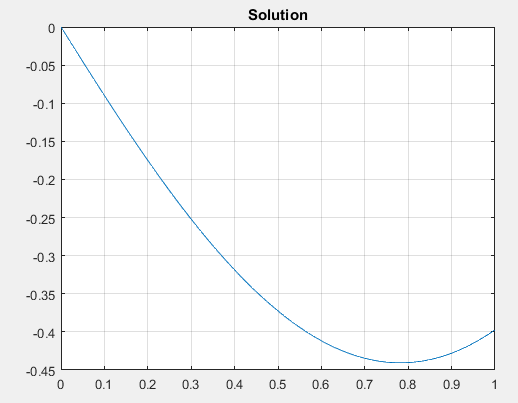
\includegraphics{./abrak/pelda_01.png}
\end{center}
Ehhez az $m = 0$ választás elegendő volt. Ezzel szemben, ha változtatunk a peremfeltételen, és az intervallum jobb oldalán a
\begin{equation*}
u'(1) = 0
\end{equation*}
feltételt követeljük meg, akkor $m=0$ esetén nincs konvergencia, és még $m=1$ esetén is problémás a helyzet, mert a Newton-iteráció nem konvergál, ezért meg kell adni kezdeti feltételt. A 
$\text{cinit} = [1]$ paraméterrel, azaz a $\Phi_1$ komponens kezdeti együtthatóját 1-re változtatva viszont már van konvergencia, és megkapjuk a megoldást:
\begin{center}
	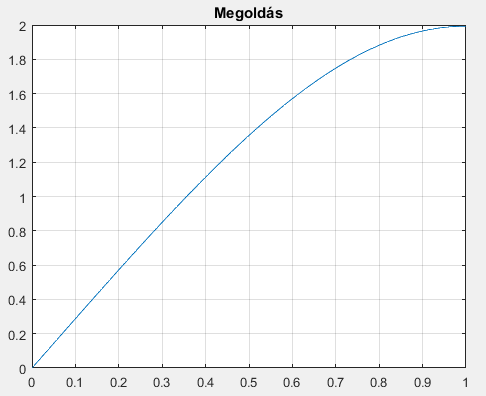
\includegraphics{./abrak/pelda_02.png}
\end{center}



%% 
 
%  Hivatkozások
\bibliography{hivatkozasok}	% TODO pontos adatok, kis-nagybetű javítások a cikkekhez % TODO kis-nagybetű bizonyos cikkeknél
\bibliographystyle{ieeetr}
 
\end{document}